%!TEX root = thesis.tex

\chapter{Introduction}
\label{chap:introduction}

Robots play an immanent role in today's world. They can be stationary, like fixed mounted industrial robot arms or mobile. They can be used to enlighten human work in many different areas. Robots are utilized for automation of production processes, medical surgery,...
Usually they are programmable, multi functional mechanical systems.
Industrial robots utilized in factories that perform repetitive tasks, high precision medical robots, household robots (automatic vacuum cleaner or lawn mower). Robots can be arbitrary intelligent - research tends to create robots that are able to act largely autonomous. Research in the branch of \emph{robotics}. Due to \citep{lavalle2006} describes the term robotics the area of automation of mechanical systems that have sensing, actuation and computation capabilities and research tends to create control software that is able to perform high-level tasks like pick and place actions on robot hardware (translate into low-level control commands, executable on the hardware). An important property of an autonomous system is it's ability to plan its motions. It should be able to move towards a target position without colliding with obstacles in it's environment. Moving the robot hand cannot follow any arbitrary trajectory towards a target pose. During that motion it might collide with itself or any other obstacle within it's environment. That means those trajectories have to be planned carefully to avoid accidental collisions and to generate smooth and well controlled robot motions. The planned paths should be preferably short and may not contain unnecessary motions. Without motion planning the motions have to be constantly specified by a human operator - not preferable, only suitable for repetitive tasks.

The design and implementation of high-level control software for a robot is a cumbersome task. The algorithms need to be tested and debugged during implementation process, but those tests come with a high level of risk. Incorrect algorithms can lead to damages on robot components or their environment and entail costly repairs. In the worst case even people can get hurt by uncontrolled robot motions. The solution to those problems is the usage of a simulator that mimics the robot components and their behavior as accurate as possible. It has to provide the same control interface to allow to test and debug each part of the software on the simulator before it gets utilized on the real robot. The usage of a simulator allows to easily test and evaluate different design approaches and algorithms during the software development process. The simulator acts as replacement for the real robot and facilitates parallelization of testing and debugging tasks. The real robot may be blocked by another person or unavailable at certain times. Working with the robot comes with an overhead(technical problems). The simulator allows to focus on implementation and debugging.

Those considerations motivated the first part of this thesis -- the realistic replication of the IIS-Lab robot setup on a suitable simulation platform. This involves the creation of an exact model of the robot setup, containing the various robot components and their environment. The necessary steps are explained in Chapter \ref{chap:simulation}.


Very often various groups of developers are working simultaneously on different parts of the software. But in most cases there is only one device that can be used for testing and so only one can run his/her code at a time. The others have to wait until they get access to the robot. Moreover, tests on real robots always come with a high level of risk. Incorrect algorithms can lead very fast to damages on robot components or their environment and entail costly repairs. In the worst case even people can get hurt by uncontrolled robot motions.



The second part of the thesis is about motion planning. Moving the robot hand cannot follow any arbitrary trajectory towards a target pose. During that motion it might collide with itself or any other obstacle within it's environment. That means those trajectories have to be planned carefully to avoid accidental collisions and to generate smooth and well controlled robot motions. This also involves to create and maintain an internal representation of the robot and it's environment, a step that is common to the simulation part of the thesis. Chapter \ref{chap:moveit} shows the configuration and integration of the motion planning framework MoveIt into the IIS-Lab robot setup along with some usage examples.

Chapter \ref{chap:pick_place} focuses on MoveIt's grasping functionality. It shows, how a reference `Pick and Place' task can be planned with the planning tools  and executed on the simulator and the real robot as well.

\section{IIS-Lab Robot Setup}
\begin{figure}[ht]
	\centering
  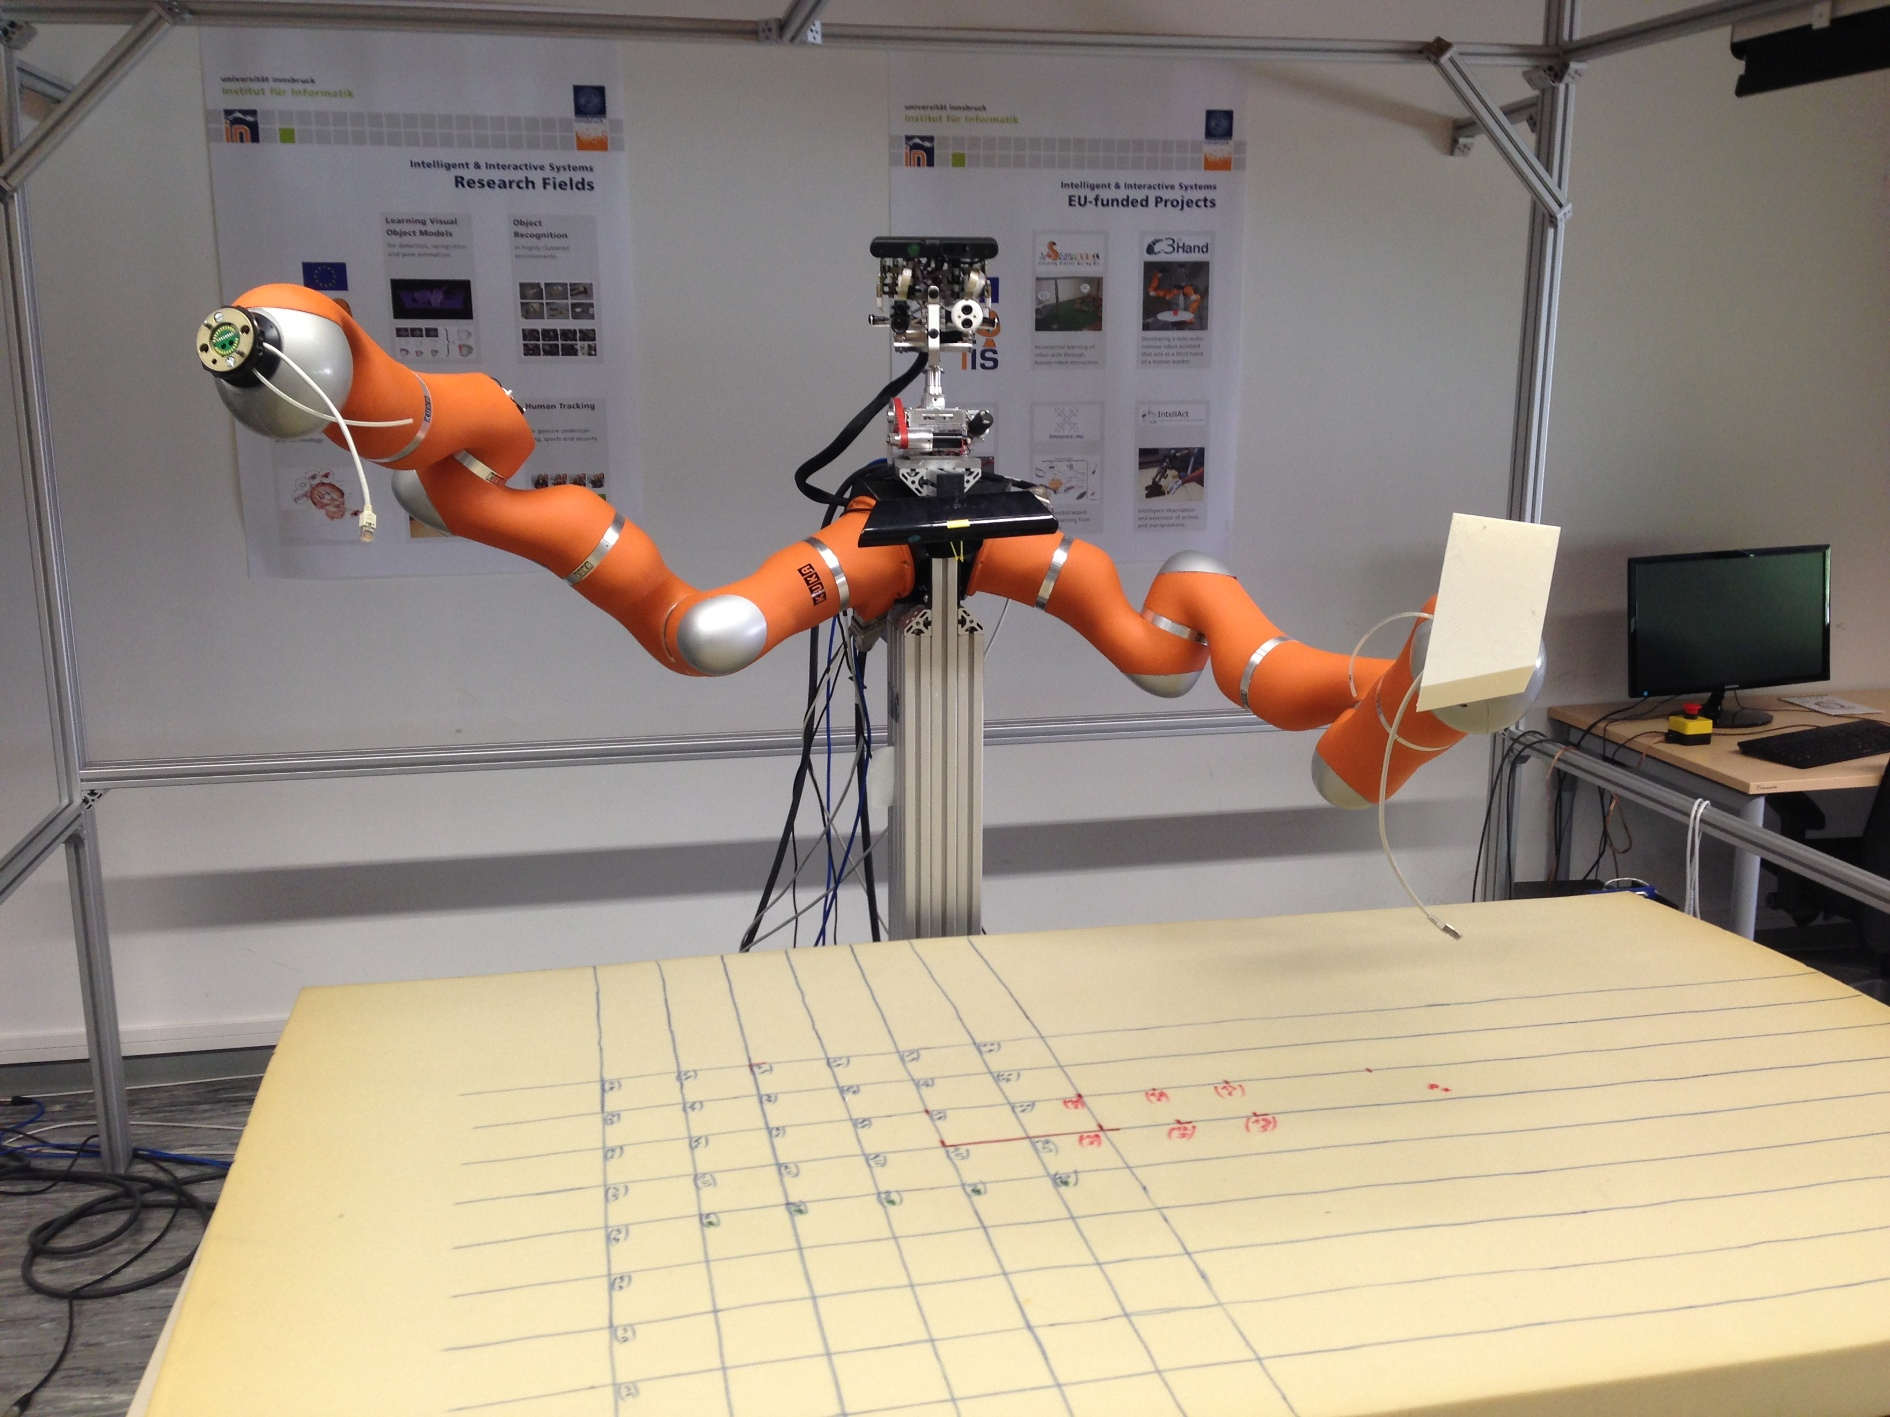
\includegraphics[width=0.75\textwidth]{images/robot_setup.jpg}
	\caption{Current setup in the IIS-Lab}
	\label{fig:iis_setup}
\end{figure}

The structure of the robot setup in the IIS lab changes frequently, as new robot components are introduced and arrangements are modified. The robot setting considered in this thesis is a snapshot but the provided solution should be customizable to reflect alternating setups. The main part of the robot setup consists of an aluminium torso with two mounted 7 DOF\footnote{Degrees of freedom - the number of independent variables, necessary to describe a robot's configuration} KUKA LWR4+ industrial robot arms, as can be seen in Figure \ref{fig:iis_setup}. The IIS lab also owns two Schunk SDH robot hands that act as end effectors. The workspace where experiments usually take place consists of a table, covered with a foam mat in front of the robot. Additionally there is a Kinect camera mounted on the torso, between both arms, that provides RGB and depth images of the task environment. The described setup is considered in the simulation and the motion planning chapters. 

\section{Project Targets}

The first goal of the project is to create a realistic replication of the IIS lab robot setup, using a suitable simulation platform. The solution needs to be able to generate proper sensor data and provide the same ROS control interface as the real robot. Additionally it would be preferable that the solution is able to detect and visualize accidental collisions of robot components with the environment. The second objective is to choose and integrate a state of the art motion planning framework into the existing setup. The required functionality includes  solving inverse kinematics problems (computing a joint configuration for a given Cartesian goal pose) up to planning and execution of trajectories for complex robot motions in joint space and Cartesian space. The proper functioning will then be shown by planning and executing a benchmark pick and place task on the simulator and the real robot as well.

The implementation of those objectives requires to determine the exact properties of the involved robot components and create kinematic, dynamic and volumetric models. This includes to do an exact measuring of the robot setup, the involved components and their placement relative to each other and create an internal representation of the world. For Cartesian positioning functionality it is also necessary to define a world reference frame and place components relative to that reference frame. \citep{craig2005} describes the inverse kinematics (IK) problem as the problem of finding possible joint settings for the robot to achieve a desired end effector position and orientation in Cartesian space. Forward kinematics (FK) is the reverse problem of finding the position and orientation of the end effector, given a set of joint angles. The end effector is the tool, mounted on the tip of the robot arm.


\section{The Robot Operating System(ROS)}

The implementation of the project requirements is based on ROS. Therefore a brief introduction about the basic concepts\footnote{http://wiki.ros.org/ROS/Concepts} shall be given here. The explained terminology will be used throughout this thesis. As stated in \cite{quigley2009}, ROS is not an operating system in the classical sense. It runs on top of a host operating system (usually linux) and can be seen as an additional communication layer, providing various mechanisms for inter process communication. A ROS system consists of a number of \emph{nodes}. Each node is an independent computation unit that runs in it's own process, adding some clearly defined functionality to the overall system. For example one node can be responsible for planning, another one for perception and a third one for controlling the hardware. Nodes communicate to each other by passing \emph{messages}, using the ROS communication infrastructure. Messages are strictly typed data structures, defined in a special message composition format\footnote{http://wiki.ros.org/msg}. They can be composed of primitive types like float, integer or string, but also of other message types. Therefore it is possible to create arbitrary complex messages for each use case. Messages are published to \emph{topics}. A topic is a strongly typed message bus, addressed by it's \emph{topic name}. Arbitrary nodes can connect to a topic in parallel, as long as they use the correct message type. Each node can publish and subscribe to a number of topics. It is also possible that various nodes publish to the same topic. 

Topic names are strings, used to identify topics. They can be organized into \emph{namespaces} to build a tree hierarchy comparable to the directory structure in a file system. This is very important, as for example the simulator should use similar topic names as the real robot. The namespace concept allows both instances to use identical names but each one in it's own namespace. The following samples represent valid topic names:
\begin{itemize}
\item \texttt{/} (this is the root namespace)
\item \texttt{/topic}
\item \texttt{/component/topic}
\item \texttt{/namespace/component/topic}
\end{itemize}

The communication via ROS topics is asynchronous - involved nodes may even not be aware of each others existence. Synchronous message exchange between nodes happens via ROS \emph{services}. In contrast to topics, a service with a given name can only be offered by one single node. Services are addressed, using the same naming strategy as topics. The service message is composed of a request and a response part. A client node that sends a service request will block, until the advertising node has handled the request and delivers a response. The concept of ROS topics and services is shown in Figure \ref{fig:ros_concept}
\begin{figure}[h]
	\centering
  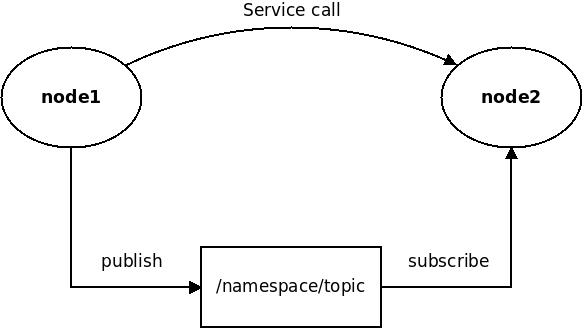
\includegraphics[width=0.5\textwidth]{images/ros_concept.jpg}
	\caption{ROS nodes, topics and services}
	\label{fig:ros_concept}
\end{figure}

The nodes of a ROS system can be distributed over various different machines. One of them has to be the dedicated \emph{ROS master}. The master is responsible to handle topic and service registrations and holds information about the involved ROS nodes. Other machines connect to the master via network. The ROS master also provides a centralized \emph{parameter server}. This is a shared dictionary that can be used to store and retrieve configuration data and other shared parameters. Nodes can access the parameter server at runtime and read or modify it's content. \\

A system usually consists of a large number of nodes that have to be configured and started. This can be done, using so called \emph{launch files}. Those are simple textfiles, holding startup information and configuration details for one or more nodes in an XML like syntax. Using the \emph{roslaunch} command line tool, a whole system of nodes can be configured and launched at once. \\

ROS is a modular software system organized into \emph{packages}. Each package adds clearly defined functionality and can be reused in other systems. Custom functionality is added to a ROS system by creating a new package and developing the required piece of software. A package might contain one or more ROS nodes or even only configuration data. Existing packages are usually installed, using a software repository package manager. A very useful ROS package is the visualization tool \emph{RViz}. This tool provides a number of different plugins that allow to display robot setups and configurations, planned trajectories or point cloud data from a vision sensor. RViz gets utilized in the motion planning related part of this project.